\subsection{Parameter Settings}
In this section, we give the parameter settings by experiments, including the threshold $\alpha$ used in the incrementally growing of medoids,
and the parameter top \emph{K} concepts used in our basic and refined algorithms. More details are as follows.

Fig.~\ref{fig:init} reports the PCC values of the refined algorithm varying with the values of $\alpha$. We can see that the PCC values first
increase to a peak value varying with the values of $\alpha$ from 0.5 to 0.78 then decrease continuously. Meanwhile, if the values of $\alpha$
vary from 0.6 to 0.78, our refined algorithm can maintain higher PCC values and the variance of PCC is no more than 0.06. In the following
experiments, we select $\alpha$ = 0.7 as an optimal value.
\begin{figure}[th]
 \centering
 \includegraphics[width=0.7\columnwidth]{parameter-a-PCC.eps}
 \caption{PCC of our basic algorithm varying with values of $\alpha$}
 \label{fig:init}
\end{figure}

Fig.~\ref{fig:topK} reports the PCC values varying with the values of top K. We can see that as the values of top \emph{K} increase, the PCC
values are first increasing then decreing. Meanwhile, if the values of top \emph{K} vary in the range of [2,5], the PCC values present a little
variance and maintain the higher values compared to other cases. In the following experiments, we select top \emph{K}=5 as an optimal value.
\begin{figure}[th]
 \centering
 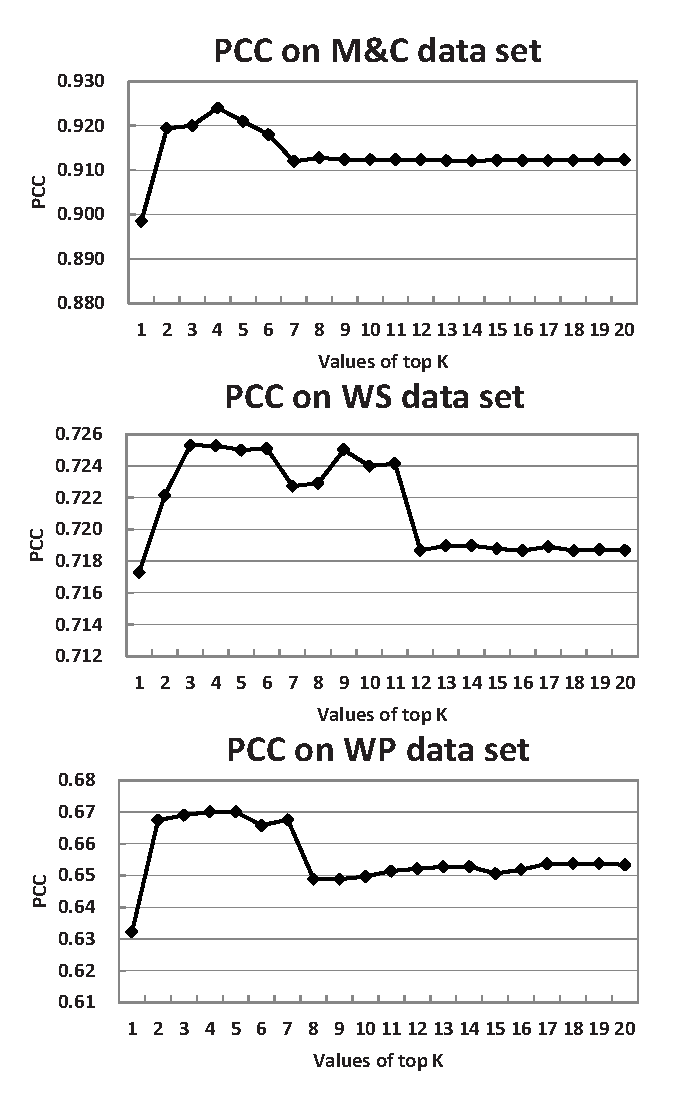
\includegraphics[width=0.7\columnwidth]{topK-allSets.eps}
 \caption{PCC of varying with values of top K}
 \label{fig:topK}
\end{figure}
